%---------------------------------------------------------------------
%   documentclass
%---------------------------------------------------------------------
\documentclass[a4paper]{article}

%---------------------------------------------------------------------
%   packages
%---------------------------------------------------------------------
\usepackage{mathtools}
\usepackage[english]{babel}
\usepackage[enc=cp1250]{hrlatex}
\usepackage[T1]{fontenc} %pekne makcene
\usepackage{lmodern} %spolu s T1 smooth font!
\usepackage{hyperref} %odkazy
\usepackage{amsmath}
\usepackage{cite} %bibtex
\usepackage{enumitem}
\usepackage{titlesec} %section titles font size change
\usepackage{color} %for \definecolor
\usepackage{colortbl} %for \rowcolor command
\usepackage{eucal} %for nice letters like \mathcal{A}
\usepackage{tikz}
\usepackage{scalefnt}

%---------------------------------------------------------------------
%   margins
%---------------------------------------------------------------------
\oddsidemargin 0.0in
\evensidemargin 0.0in
\textwidth 6.1in
\textheight 23.94cm
\topmargin -0.35in

%---------------------------------------------------------------------
%   various settings
%---------------------------------------------------------------------
\pgfrealjobname{research} % <-- NOTE: this needs to be the real document's basename
                        %     (else you'll only get an empty output file)

\newif\ifmine % introduce a switch for draft vs. final document
\minetrue

\newif\iffinal % introduce a switch for draft vs. final document
\finaltrue % use this to compile the final document
\iffinal
  \newcommand{\inputTikZ}[1]{%
    \input{#1.tikz}%
  }
\else
  \newcommand{\inputTikZ}[1]{%
    \beginpgfgraphicnamed{#1-external}%
    \input{#1.tikz}%
    \endpgfgraphicnamed%
  }
\fi

\setlist{nolistsep} %so that lists have normal spacing

\titleformat{\section}{\LARGE\bfseries}{\thesection}{1em}{} %section titles
\titleformat{\subsection}{\Large\bfseries}{\thesubsection}{1em}{} %subsection titles

\definecolor{tablehead}{RGB}{238,233,233} %nice smooth grey

\setlength{\parindent}{0pt} %we don't need no indentation

\graphicspath{{./pics/}} %picture dir

%---------------------------------------------------------------------
%   environments
%---------------------------------------------------------------------
\renewenvironment{abstract}[1]
{
	\Large
	\begin{center}
		\textbf{#1}
	\end{center}
	
	\normalsize
	
	\addtolength{\leftskip}{1in}
	\addtolength{\rightskip}{1in}
	\setlength{\parindent}{0in}
}
{
}

\newenvironment{itemizesp}
{
    \begin{itemize}
}
{
    \end{itemize}
}

\newcommand{\deftoken}{\boldmath{$\mathcal{DEFINITION}$}}
\newcommand{\restoken}{\boldmath{$\mathcal{RESULT}$}}
\newcommand{\dotoken}{\boldmath{$\mathcal{DO METHOD}$}}
\newcommand{\textbff}[1]{{\large \textbf{#1}}}

%---------------------------------------------------------------------
%   magic code
%---------------------------------------------------------------------
% Here it is: the code that adjusts justification and spacing around caption.
\makeatletter
% http://www.texnik.de/floats/caption.phtml
% This does spacing around caption.
\setlength{\abovecaptionskip}{6pt}   % 0.5cm as an example
\setlength{\belowcaptionskip}{6pt}   % 0.5cm as an example
% This does justification (left) of caption.
\long\def\@makecaption#1#2{%
  \vskip\abovecaptionskip
  \sbox\@tempboxa{#1: #2}%
  \ifdim \wd\@tempboxa >\hsize
    #1: #2\par
  \else
    \global \@minipagefalse
    \hb@xt@\hsize{\box\@tempboxa\hfil}%
  \fi
  \vskip\belowcaptionskip}
\makeatother

%---------------------------------------------------------------------
%   document
%---------------------------------------------------------------------
\begin{document}
    \thispagestyle{empty}
    %---------------------------------------------------------------------
    %   topmatter
    %---------------------------------------------------------------------
    \title{\textbf{Distance oracles for timetable graphs - research}}
    \author{Franti�ek Hajnovi� \\
    Faculty of Mathematics, Physics and Informatics \\
    Comenius University \\
    Bratislava, Slovakia \\
    \texttt{ferohajnovic@gmail.com}}
    \date{April 2012}
    \maketitle

    \vskip 0.5cm

    %---------------------------------------------------------------------
    %   abstract
    %---------------------------------------------------------------------
    \begin{abstract}{Abstract}
        In this paper, we would like to summarize the work done on distance oracles, shortest path queries and shortest timetable connection queries. The list of papers is not comprehensive, but offers a good look into the state of research in this area. \\

		Keywords: \textbf{distance oracles}, \textbf{timetable graphs}, \textbf{shortest path}
 	\end{abstract}	

    \begin{center}
        \line(1, 0) {450}
    \end{center}

    \textbf{Declaration:} This paper is just a summary of the listed articles and the ideas presented are all coming from the respective article being summarized. I re-explain several points deemed important for the purposes of this research. At times, I borrow the exact words of the authors of the article at question.

    \begin{center}
        \line(1, 0) {450}
    \end{center}

    %---------------------------------------------------------------------
    %   list of papers
    %---------------------------------------------------------------------
    \section{List of considered papers}
        \textbf{Distance labeling: }
        \begin{enumerate}
            \item \ref{subsec:distlabel} Distance Labeling in Graphs ~\cite{distlabel04}
            \item \ref{subsec:2hop} Reachability and distance queries via 2-hop labels ~\cite{2hop03}
        \end{enumerate}
        \hspace*{\fill}

        \textbf{Distance oracles: }
        \begin{enumerate}
            \item \ref{subsec:apxdo} Approximate Distance Oracles ~\cite{apxdo05}
            \item \ref{subsec:exactplanar} Exact Distance Oracles for Planar Graphs ~\cite{exactplanar10}
            \item \ref{subsec:fsensitivity} f-Sensitivity Distance Oracles and Routing Schemes ~\cite{fsensitivity10}
            \item \ref{subsec:linkfailure} Improved Distance Oracles for Avoiding Link-Failure ~\cite{linkfailure02}
            \item \ref{subsec:powerlaw} A Compact Routing Scheme and Approximate Distance Oracle for Power-Law Graphs ~\cite{powerlaw09}
            \item \ref{subsec:ramseyphd} Ramsey Partitions Based Approximate Distance Oracles ~\cite{ramseyphd08}
            \item \ref{subsec:sketchbased} A Sketch-Based Distance Oracle for Web-Scale Graphs ~\cite{sketchbased10}
            \item \ref{subsec:sommerthesis} Approximate Shortest Path and Distance Queries in Networks ~\cite{sommerthesis10}
            \item \ref{subsec:sparse} Distance Oracles for Sparse Graphs ~\cite{sparse09}
            \item \ref{subsec:spatialnetw} Distance Oracles for Spatial Networks ~\cite{spatialnetw09}
        \end{enumerate}
        \hspace*{\fill}

        \textbf{Route-planning: }
        \begin{enumerate}
            \item \ref{subsec:contracthier} Contraction Hierarchies: Faster and Simpler Hierarchical Routing in Road Networks ~\cite{contracthier08}
            \item \ref{subsec:engineeringroute} Engineering Route Planning Algorithms ~\cite{engineeringroute09}
            \item \ref{subsec:highwaydim} Highway Dimension, Shortest Paths, and Provably Efficient Algorithms ~\cite{highwaydim10}
            \item \ref{subsec:hwhierarchies} Highway Hierarchies Hasten Exact Shortest Path Queries ~\cite{hwhierarchies05},
            \item \ref{subsec:routeplandiz} Route Planning in Road Networks ~\cite{routeplandiz08}
            \item \ref{subsec:transit} TRANSIT Ultrafast Shortest-Path Queries with Linear-Time Preprocessing~\cite{transit06}
            \item \ref{subsec:transithh} In Transit to Constant Time Shortest-Path Queries in Road Networks ~\cite{transithh}
        \end{enumerate}
        \hspace*{\fill}

        \textbf{Time-dependent routing: }
        \begin{enumerate}
            \item \ref{subsec:sharc} Time-Dependent SHARC-Routing ~\cite{sharc08}
            \item \ref{subsec:tchbasicalgideas} Time Dependent Contraction Hierarchies - Basic Algorithmic Ideas ~\cite{tchbasicalgideas08}
            \item \ref{subsec:timedepch} Time-Dependent Contraction Hierarchies ~\cite{timedepch09}
        \end{enumerate}
        \hspace*{\fill}

        \textbf{Timetables related: }
        \begin{enumerate}
            \item \ref{subsec:compshpathapp} Experimental comparison of shortest path approaches for timetable ~\cite{compshpathapp04}
            \item \ref{subsec:engtimeexp} Engineering Time-Expanded Graphs for Faster Timetable Information ~\cite{engtimeexp09}
            \item \ref{subsec:multilevelgr} Using Multi-level Graphs for Timetable Information in Railway Systems ~\cite{multilevelgr02}
            \item \ref{subsec:timetablemodelsalgs} Timetable Information: Models and Algorithms ~\cite{timetablemodelsalgs07}
        \end{enumerate}
        \hspace*{\fill}

        \textbf{Others: }
        \begin{enumerate}
            \item \ref{subsec:complexnetw} Complex networks: small-world, scale-free and beyond ~\cite{complexnetw03}
        \end{enumerate}
        \hspace*{\fill}

        \textbf{Unclassified: }
        \begin{enumerate}
            \item \ref{subsec:reachforastar} Reach for A*: Efficient Point-to-Point Shortest Path Algorithms ~\cite{reachforastar06}
            \item \ref{subsec:twoworlds} Car or Public Transport--Two Worlds ~\cite{twoworlds09}
        \end{enumerate}
        \hspace*{\fill}

    %---------------------------------------------------------------------
    %   paper summaries
    %---------------------------------------------------------------------
    \pagebreak
    \section{Distance labeling}

        \subsection{Distance Labeling in Graphs}
        \label{subsec:distlabel}

        \textbff{Author(s): }
        \begin{itemizesp}
            \item Cyril Gavoille
            \item David Peleg
            \item St�phane P�rennes
            \item Ran Raz
        \end{itemizesp}
        \textbff{Year: }2004 \\
        \textbff{Institution(s): }
        \begin{itemizesp}
            \item Universit� Bordeaux
            \item The Weizmann Institute of Science, Israel
            \item Universit� de Nice-Sophia Antipolis
        \end{itemizesp}
        {\hfill}\\
        \textbff{Concern:} The paper considers the problem of \emph{distance labeling in graphs}. Distance labeling itself is an approach that assigns each node of the graph some label in such a way, that queries for distance between any pair of vertices can be answered using only the information provided by the labels. This paper talks about various lower and upper bounds on the length of such labels for individual classes of graphs, as well as \emph{time complexity of the extraction of the distance} from the labels. \\
        {\hfill}\\
        \textbff{Outline:} After some necessary \textbf{definitions} and short mention of the \textbf{related work}, the results concerning \textbf{upper bounds} (sufficient sizes of labels) are presented. Those include an upper bound for general graphs and graphs with a given separator. Next, \textbf{lower bounds} are provided for general graphs, graphs with a given separator, planar graphs and trees, most of the results obtained by a generalized theorem proven before. Finally, in the last section, the \textbf{time complexity of extracting the actual distance} from the labels is considered, and shown to be too high for practical use for some extreme cases in the class of general graphs.\\

        We should note, that we may think of distance labeling as of some form of distance oracle based method. Obtaining the labels requires some preprocessing time and results in the labels, that together take some space (size of the DO) . Query time is equivalent to the distance decoding (see below). Thus it is just a different (a bit more restricted) approach to the same thing. Let us look closer at the results obtained.\\

        \def\defdistlab{\textbf{Distance labeling} $<L, \mathnormal{f}>$ for a graph $G$ consists of \textbf{node labeling} $L$ and \textbf{distance decoder} $\mathnormal{f}$. The first is a function that assigns each node a label. Second is a function that computes the distance between the nodes, given their labels. $<L, \mathnormal{f}>$ is a \textbf{distance labeling scheme} for family (class) of graphs $\mathcal{G}$ if it is a correct distance labeling for every $G \in \mathcal{G}$.}\defdistlab \\

        Now we are interested in such a distance labeling scheme, that minimizes the maximal label length in all graphs of the given graph family. The obtained results are given in the table~\ref{tab:distlab}. \\

        \begin{table}[h!]
            \caption{\label{tab:distlab} Results of ~\cite{distlabel04} on the necessary length of labels. In each entry we consider a $n$-vertex subclass of the given class}
            \small
            \begin{tabular}{c|c|c}
                %legend
                \hline
                    \rowcolor{tablehead}
                    \textbf{Class of graphs} & \textbf{Lower bound} & \textbf{Upper bound} \\
                %data
                \hline
                    general & $n/2 - O(1) = \Omega(n)$ & $11n + O(\log n \log\log n) = O(n)$ \\
                    unweighted binary trees & $\log^{2} n/8 - O(\log n) = \Omega(\log^{2} n)$ & \\
                    binary trees with integral weights up to M & $\theta((\log M + \log n)\log n)$ & $\theta((\log M + \log n)\log n)$ \\
                    planar & $\Omega(n^{1/3})$ &  \\
                    bounded degree & $\Omega(\sqrt{n})$ & \\
                    having $r(n)-separator$ & $\sum_{labels} = \Omega(r(n)(n - r(n)) - 2n \log n)$ & $O(R(n) \log n + \log^{2} n)$ \\
            \end{tabular}
            \normalsize
        \end{table}

        \def\resseparator{There exists an exact distance labeling scheme with the overall size $O(n R(n) \log n + n \log^{2} n)$ and distance computing in $O(\log n)$ time for a graph having $r(n)-separator$}

        Note: In the last row (of table \ref{tab:distlab}), \def\defbigrn{$R(n) = \sum^{\log_{3/2} n}_{i=0} r(n(2/3)^i)$}\defbigrn. \def\defseparator{We say a graph class $\mathcal{G}$ has a {\boldmath$r(n)-separator$} if for every connected graph $G \in \mathcal{G}$ of $n$ vertices there is a separator of size at most $r(n)$ such that upon its deletion we obtain components that are again graphs from $\mathcal{G}$. Moreover, all of these created components have size at most $r(2n/3)$.}\defseparator\\

        Other results are concerning the time complexity of the distance decoder. The main result is rather technical, so we'll demonstrate it on a simpler corollary: \\

        \def\restimelabelgeneral{Let $\mathcal{G}$ be the family of all graphs. For infinitely many $n$, we have a $G \in \mathcal{G}$, for which:
        \begin{enumerate}
            \item There is an exact (with stretch $1$) distance labeling scheme with maximal label $\leq 3\log n + o(\log n)$.
            \item However, for any distance labeling scheme with stretch $< 2$ that satisfies $\sum_{u \in V(G)} |L(u, G)| \leq n^{2} / 2 - O(n \log n)$ (that is also the one from point 1.)), the time and space complexities of distance decoder function $f$ are larger than any constant size stack of exponentials ($2^{2^{\dots^{2^{n}}}}$ - constant height of the power stacking).
        \end{enumerate}}\restimelabelgeneral
        {\hfill}\\

        Put informally, for almost any size of graph, there is such graph for which we can find a labeling producing only short labels. But for that graph, there will not be any distance labeling scheme that would answer distance queries in a small time/space complexity.

        \begin{figure}[h!]
            \scriptsize
            \begin{center}
                \inputTikZ{./tikzpics/separator}
            \end{center}
            \caption{\label{fig:distanceseparator} Graph has a recursive $3$-separator (so $r(n)$ is constant in this case): None of the components, after removing the separator $r_1$, contains more than $2/3 n$ vertices. This holds recursively (e.g. after removing the separator $r_2$, the green areas are not too large with respect to $Z$). There is no $1$-separator, however, as there is no way to decompose area $Z$ with separator of size one in a mentioned balanced manner.}
        \end{figure}

        \subsection{Reachability and distance queries via 2-hop labels}
        \label{subsec:2hop}

        \textbff{Author(s): }
        \begin{itemizesp}
            \item Edith Cohen
            \item Eran Halperin
            \item Haim Kaplan
            \item Uri Zwick
        \end{itemizesp}
        \textbff{Year: }2002 \\
        \textbff{Institution(s): }
        \begin{itemizesp}
            \item AT\&T Labs Research
            \item Tel-Aviv University
        \end{itemizesp}

    \pagebreak
    \section{Distance oracles}

        \subsection{Approximate Distance Oracles}
        \label{subsec:apxdo}

        \textbff{Author(s): }
        \begin{itemizesp}
            \item Mikkel Thorup
            \item Uri Zwick
        \end{itemizesp}
        \textbff{Year: } 2004 \\
        \textbff{Institution(s): }
        \begin{itemizesp}
            \item AT\&T Labs Research
            \item Tel-Aviv University
        \end{itemizesp}
        {\hfill}\\
        \textbff{Concern:} Thorup and Zwick provided an important result in this paper, which is further mentioned in other works in the distance oracle area. \def\resthzwck{They showed, that given an undirected weighted graph of $n$ vertices and $m$ edges and a chosen integer $k \geq 1$, we can build a distance oracle answering shortest path queries, the oracle having following properties:
        \begin{itemizesp}
            \item preprocessing takes $O(kmn^{1/k})$ expected time
            \item resulting distance oracle is of size $O(kn^{1 + 1/k})$
            \item answering queries takes $O(k)$ time
            \item stretch of the anwser(i.e. the worst ratio of returned path against the optimal value) is $2k - 1$ at most
        \end{itemizesp}}\resthzwck
        {\hfill}\\
        \textbff{Outline:} First, there is a brief \textbf{history of the work done} in the area up to the date (2004) and a summary of known methods at that time, compared to the distance oracle of Thorup and Zwick. Following is the presentation of an \textbf{approximate distance oracle for metric spaces}, whose preprocessing time is \emph{expeceted} $\mathcal{O}(n^2)$, due to the randomized nature of the preprocessing algorithm. The \textbf{derandomization} (with a slight loss in efficiency) follows and the \textbf{adjustment} is made for graphs not explicitly embedded in a metric space. In the final section, there is an argument based on the girth conjecture stating that the distance oracle of Thorup and Zwick is \textbf{essentially optimal} with regard to amount of storage needed. \\
        {\hfill}

        The result of Thorup and Zwick says, that we can make compromises - by increasing preprocessing time and the size of the DO, we can achieve better stretch and query time, and vice versa. Note, however, that only values of $k$ up to $\log n$ (when preprocessing and size of DO reach their minimum) are desirable, higher values of $k$ already increase all the factors. Also note, that increasing query time does not increase the accuracy, which is a bit counterintuitive. Christian Sommer's DO-based method (see ~\ref{subsec:sommerthesis}) achieves different kind of trade-offs. \\

        \begin{figure}[h]
            \scriptsize
            \begin{center}
                \inputTikZ{./tikzpics/thorupcompromises}
            \end{center}
            \caption{\label{fig:apxdocompromises} Possible trade-offs among preprocessing time, size of DO, query time and stretch}
        \end{figure}

\ifmine
        \textbff{Lower bound on space} \\

        Let us concisely describe, why the proposed distance oracle is essentially optimal, as it is an interesting discussion. First, we need a few definitions. \def\defspanner{A \textbf{$t$-Spanner} is a subgraph of a graph, that preserves distances between any pair of vertices up to the factor of $t$}\defspanner . In other words - any distance in the $t$-spanner is at most $t$ times the distance in the original graph. We should note, that we consider only subgraphs whose set of vertices is the same as in the original graph. \\

        Next, we have the \def\defgirth{\textbf{girth} of a graph, which is the size of its smallest cycle}\defgirth . There is a close relation between spanners and girth of a graph: \\

        \textbf{Theorem 1:} \def\resspangirth{the girth of a graph is at least $t+2$ $\iff$ no \emph{proper} subgraph of it is a $t$-spanner}\resspangirth\\

        which is trivial to prove. Another result states: \\

        \textbf{Theorem 2:} \def\resgirthtwok{every $n$-vertex graph with at least $n^{1 + 1/k}$ edges contains a cycle of size $\leq 2k$, thus is of girth at most $2k$}\resgirthtwok . \\

        Combining the two theorems, we have: \\

        \begin{enumerate}
            \item $n$-vertex graph with $n^{1 + 1/k}$ edges $\Rightarrow$ girth at most $2k$ (from the second theorem)
            \item girth at most $(2k - 1) + 1$ $\Rightarrow$ $\exists$ $(2k - 1)$-spanner (from the first theorem, where $t = (2k - 1)$)
        \end{enumerate}
        {\hfill}

        Thus we can conclude: \\

        \textbf{Theorem 3:} \def\reseveryspanner{every graph on $n$ vertices has a $(2k - 1)$-spanner with $\mathcal{O}(n^{1 + 1/k})$ edges}\reseveryspanner \\

        If the original graph is sparse enough, we can take it whole as a spanner, otherwise we apply the two mentioned implications. \\

        The discussion above was concerning undirected and unweighted graphs. However, the last result is valid for weighted graphs as well. We need to extend the definitions of $t$-spanner and girth - the extension of the definition of a $t$-spanner for weighted graphs is straightforward and girth stays defined the way it was (that is - the size, i.e. the number of edges of the smallest cycle). The first theorem will no longer hold, however, the necessary right-to-left implication used in point 2. above (where we actually use the inverse of that implication) will still be valid (from any cycle, we can simply remove the most expensive edge while not increasing any distance by the factor more than $(2k - 1)$). The second theorem used is not affected by the graph being weighted. Thus the conclusion we drew for unweighted graphs holds for weighted graphs as well. \\

        However, it is conjectured by Erd\"{o}s (and others as well), that \\

        \textbf{Conjecture 1:} \def\reserdos{for any $k \geq 1$ there are graphs with $\Omega(n^{1 + 1/k})$ edges and girth greater than $2k$}\reserdos \\

        The $2k$ can actually be pushed even more to $2k + 1$, if we realize, that any graph contains a bipartite graph with at least half the edges. Thus we can obtain a graph with all cycles of an even size and still satisfying $|E| = \Omega(n^{1 + 1/k})$. \\

        Combining theorem 1 and the conjecture, and repeating theorem 3, we have: \\

        \begin{enumerate}
            \item $\exists$ graph $G$ of $n$ vertices with $\Omega(n^{1 + 1/k})$ edges, no proper subgraph of which is a $2k - 1$-spanner (conjecture and theorem 1)
            \item $G$ is a graphs of $n$ vertices $\Rightarrow$ $G$ has a $(2k - 1)$-spanner with $\mathcal{O}(n^{1 + 1/k})$ edges (theorem 3)
        \end{enumerate}
        {\hfill}

        Thus it is shown, that for a $(2k - 1)$-spanner $\Omega(n^{1 + 1/k})$ edges are \textbf{sufficient}, though the same amount of edges is \textbf{necessary} for some cases (in number 1., we would have to take the whole graph as a spanner). As written in the article, any distance oracle capable of producing paths witnessing the estimated distances must explicitly or implicitly contain an appropriate spanner. Thus provided that the conjecture holds, the size of any distance oracle with stretch $2k - 1$ is $\Omega(n^{1 + 1/k})$. \\

        The final argument above is a bit high-level, and a different one, more formal is provided in the article. Also, the full optimality was not achieved, as the space complexity of the algorithm of Thorup and Zwick was expressed in words, rather than in bits, leaving a logarithmic gap.
\fi

        \subsection{Exact Distance Oracles for Planar Graphs}
        \label{subsec:exactplanar}

        \textbff{Author(s): }
        \begin{itemizesp}
            \item Shay Mozes
            \item Christian Sommer
        \end{itemizesp}
        \textbff{Year: }2011 \\
        \textbff{Institution(s): }
        \begin{itemizesp}
            \item Brown University
            \item MIT
        \end{itemizesp}

        \subsection{f-Sensitivity Distance Oracles and Routing Schemes}
        \label{subsec:fsensitivity}

        \textbff{Author(s): }
        \begin{itemizesp}
            \item Shiri Chechik
            \item Michael Langberg
            \item David Peleg
            \item Liam Roditty
        \end{itemizesp}
        \textbff{Year: }2011 \\
        \textbff{Institution(s): }
        \begin{itemizesp}
            \item The Weizmann Institute of Science
            \item Open University of Israe
            \item Bar-Ilan University
        \end{itemizesp}

        \subsection{Improved Distance Oracles for Avoiding Link-Failure}
        \label{subsec:linkfailure}

        \textbff{Author(s): }
        \begin{itemizesp}
            \item Rezaul Alam Chowdhury
            \item Vijaya Ramachandran
        \end{itemizesp}
        \textbff{Year: }2002 \\
        \textbff{Institution(s): } The University of Texas at Austin \\
        \hspace*{\fill}\\
        \textbff{Concern:} Paper attempts to solve the problem of preprocessing an edge-weighted \textbf{directed} graph to answer queries for shortest path avoiding specific link. \\

        \textbff{Outline:} \textbf{Introduction }and \textbf{necessary notations} are followed by the presentation of the two algorithms - DT-1 and DT-2 - that are later upgraded in the paper. CR-1 and CR-2 - the \textbf{constructed algorithms} are proposed, each with a code listing, preprocessing description and a justification of correctness. \\

        Two functions are considered:
        \begin{itemize}
          \item $distance(x, y, u, v)$ - shortest distance from $x$ to $y$ avoiding edge $(u, v)$.
          \item $path(x, y, u, v)$ - shortest path from $x$ to $y$ avoiding edge $(u, v)$.
        \end{itemize}
        \hspace*{\fill}

        Assumption is that the time between two successive link failures are long enough to compute a new data structure in the background. \\

        The authors build upon algorithms $DT-1$ and $DT-2$ presented in paper by Demetrescu and Thorup. Those are not very complicated - $DT-1$ divides each shortest path from $x$ to $y$ to $O(\log n)$ segments, storing shortest distance from $x$ to $y$ avoiding each of these segments in a table. $DT-2$ divides each shortest-path tree $T(x)$ into $O(\sqrt n)$ bands of independent paths. Again, shortest distance avoiding these bands are precomputed. \\

        The algorithms introduced in this paper are called $CR-1$ and $CR-2$. Their respective properties are shown in the table below.

        \begin{table}[h]
            \caption{Results of ~\cite{linkfailure02}}
            \small
            \begin{tabular}{c|c|c|c}
                %legenda
                \hline
                    \rowcolor{tablehead}
                    \textbf{Algorithm} & \textbf{Preprocessing time} & \textbf{Space} & \textbf{Query time}
                %data
                \\ \hline
                    $CR-1$ & $O(mn^2 \log n + n^3 \log^2 n)$ & $O(n^2 \log n)$ & $O(1)$ \\
                    $CR-2$ & $O(mn \log^2 n + n^2 \log^3 n)$ & $O(n^2 \log^2 n)$ & $O(\log n)$ \\
            \end{tabular}
            \normalsize
        \end{table}

        \subsection{A Compact Routing Scheme and Approximate Distance Oracle for Power-Law Graphs}
        \label{subsec:powerlaw}

        \textbff{Author(s): }
        \begin{itemizesp}
            \item Wei Chen
            \item Christian Sommer
            \item Shang-Hua Teng
            \item Yajun Wang
        \end{itemizesp}
        \textbff{Year: } 2009\\
        \textbff{Institution(s): }
        \begin{itemizesp}
            \item Microsoft Research
            \item MIT
        \end{itemizesp}

        %TODO
        %   comparison to Sommer's thesis
        %   approach

        \subsection{Ramsey Partitions Based Approximate Distance Oracles}
        \label{subsec:ramseyphd}

        \textbff{Author(s): } Chaya Fredman \\
        \textbff{Year: }2008 \\
        \textbff{Institution(s): } The Open University Of Israel \\

        \subsection{A Sketch-Based Distance Oracle for Web-Scale Graphs}
        \label{subsec:sketchbased}

        \textbff{Author(s): }
        \begin{itemizesp}
            \item Atish Das Sarma
            \item Sreenivas Gollapudi
            \item Marc Najork
            \item Rina Panigrahy
        \end{itemizesp}
        \textbff{Year: }2010 \\
        \textbff{Institution(s): }
        \begin{itemizesp}
            \item Microsoft Research
            \item Georgia Institute of Technology
        \end{itemizesp}
        \hspace*{\fill} \\
        \textbff{Concern:} This paper considers real-world large-scale graphs, like web graph or social networks, and tries to provide algorithms to answer shortest path queries that would be efficient and giving accurate enough results at the same time. \\

        \textbff{Outline:} A \textbf{summary of related methods} is presented at the beginning. Next, the \textbf{algorithm is described} (Online-Common-Seed), subsequently \textbf{extended to directed graphs}. Finally, \textbf{experiments} on a crawl of the web are performed, comparing the algorithm to the Bourgain's method. \\

        The provided algorithm looks the following in the preprocessing phase: \\

        \begin{equation*}
            SAMPLING \xrightarrow{\log |V| \; times} \forall u \in V: \; SAMPLE[u] \xrightarrow{k \; times} \forall u \in V: \; SKETCH[u]
        \end{equation*}
        \hspace*{\fill}

        {\boldmath$SAMPLING$} is just picking random vertices (seeds) from $V$. {\boldmath$SAMPLE[u]$} for some $u \in V$ is a set of couples $(w_i, \delta_i)$ where $w_i$ is the closest seed to $u$ from a given sampling, and $\delta_i$ is its distance from $u$. Sampling is done $\log |V|$ times - starting with $1$ sampled seed and doubling each subsequent time. Finally, {\boldmath$SKETCH[u]$} is a union of $SAMPLE[u]$ created when we iterated the whole process $k$ times. \\

        The \textbf{preprocessing }thus takes $O(k \cdot n^2)$, using one breath-first search from each seed set.

        The algorithm {\boldmath$ONLINE-COMMON-SEED(x, y)$} for answering queries compares the two $SKETCH$es of the two vertices and finds a command seed $s$, which minimizes the distance $d(x, s) + d(s, y)$. In case of no common seed, we output $\infty$. This algorithm always gives upper bound on actual shortest distance. \\

        Further, there is a proof that for $k=\Theta (n^{1/c}polylog(n))$, we get a $2c - 1$ approximation of the actual distance with high probability. \\

        Another algorithm called {\boldmath$ONLINE-BOURGAIN(x, y)$} is mentioned, since {\boldmath$ONLINE-COMMON-SEED(x, y)$} is later compared to it. {\boldmath$ONLINE-BOURGAIN(x, y)$} provides a lower bound on the actual distance. Unlike $ONLINE-COMMON-SEED$, it takes a maximum of $|d(x, S) - d(y, S)| \; \forall S$ where $S$ are seed sets from $SAMPLING$. Again, a similar theorem applies: for $k=\Theta (n^{1/c})$, we get a $O(2c - 1)$ approximation of the actual distance with high probability. \\

        Both algorithms answer queries with time complexity $O(\log n)$. \\

        Algorithms are also modified to directed graphs. \\

        Experiments were run on a large crawl of the web graph, containing about $65 000 000$ web pages and $420 000 000$ distinct URLs. For $k=1$ (guaranteed approximation of only $\log n$) they still obtained $1.2$ approximation ratio with $ONLINE-COMMON-SEED$ and $2.14$ ratio with $ONLINE-BOURGAIN$, thus showing that the theoretical guarantee could be possibly improved.

        \subsection{Approximate Shortest Path and Distance Queries in Networks}
        \label{subsec:sommerthesis}

        \textbff{Author(s): } Christian Sommer \\
        \textbff{Year: }2010 \\
        \textbff{Institution(s): } The University of Tokyo\\
        {\hfill}\\
        \textbff{Concern:} In his PhD thesis, Christian Sommer investigates the problem of \emph{efficiently computing exact and approximate shortest path queries} in graphs. Apart from that, the thesis gives a clear understanding of the problematics, terminology and related work in the area. \\

        \textbff{Outline:} A very well organized thesis begins with plenty of \textbf{motivation}, continues with extensive \textbf{definitions} and \textbf{summary} of work done on shortest path query processing. The \textbf{three main results} are then devoted a chapter, each beginning with an introduction and ending with a conclusion and open points.\\

        The thesis provides three \emph{main results}: \\
        \begin{enumerate}
            \item There is no exact DO for sparse general graphs, that would be of size $O(m)$ and have a constant query time. More specifically, given query time $t$ and multiplicative stretch $\alpha$, a required space for an exact DO is $n^{1 + \Omega(1/\alpha t)}$.
            \item Adapting the DO of Thorup and Zwick (~\cite{apxdo05}) and adjusting it for power-law graphs. The adjustment takes advantage of the high-degree nodes in power-law graphs and selects them for \emph{landmarks} in the algorithm. A theoretical proof shows why such an approach yields a good heuristics, efficiently approximating shortest paths e.g. in Internet-like topologies.
            \item An approximation DO for general undirected graphs with positive edge weights is presented. Based on random sampling and graph Voronoi duals, it provides good theoretical trade-offs between stretch and preprocessing and query times (stretch against the two). Even better is the performance in practice. Compared to DO of Thorup and Zwick, it offers a different type of trade-off: stretch of the answer is reduced when a longer query time is allowed.
        \end{enumerate}

        %TODO
        %   open points
        %   more detail
        %   comparison with article subsec:powerl (microsoft)

        \subsection{Distance Oracles for Sparse Graphs}
        \label{subsec:sparse}

        \textbff{Author(s): }
        \begin{itemizesp}
            \item Christian Sommer
            \item Elad Verbin
            \item Wei Yu
        \end{itemizesp}
        \textbff{Year: }2009 \\
        \textbff{Institution(s): }
        \begin{itemizesp}
            \item The University of Tokyo and NII
            \item Tsinghua University
        \end{itemizesp}

        \subsection{Distance Oracles for Spatial Networks}
        \label{subsec:spatialnetw}

        \textbff{Author(s): }
        \begin{itemizesp}
            \item Jagan Sankaranarayanan
            \item Hanan Samet
        \end{itemizesp}
        \textbff{Year: }2009 \\
        \textbff{Institution(s): } University of Maryland \\

    \pagebreak
    \section{Route-planning}

    \subsection{Contraction Hierarchies: Faster and Simpler Hierarchical Routing in Road Networks}
        \label{subsec:contracthier}

        \textbff{Author(s): }
        \begin{itemizesp}
            \item Robert Geisberger
            \item Peter Sanders
            \item Dominik Schultes
            \item Daniel Delling
        \end{itemizesp}
        \textbff{Year: }2008 \\
        \textbff{Institution(s): }
        \begin{itemizesp}
            \item Universitat Karlsruhe
        \end{itemizesp}
        {\hfill}\\
        \textbff{Concern:} Yet another technique is presented for answering shortest-path queries in road-networks. The idea is based on the notion of contraction. The graph is iteratively contracted, to obtain a set of shortcuts. A special version of bidirectional Dijkstra's algorithm is then run on the enhanced graph to obtain very good speed-up of 4 orders of magnitude against the classical Dijkstra's algorithm.\\

        \textbff{Outline:} The \textbf{idea is sketched} at the beginning, a brief comparisons to \textbf{related work} (mostly to Highway hierarchies and Transit-node routing) are made. The \textbf{preprocessing phase} is described, mostly the heuristics that determine the node ordering in the contraction process. \textbf{Query computation} itself is explained, some \textbf{experiments} carried out. The \textbf{conclusion} gives directions for future improvements and research.\\

        The \textbf{contraction} of a node means, that we remove it from the graph and add edges (\textbf{shortcuts}) between some of the pairs of its neighbors, so that we preserve all the distances of the original graph. Thus if the contracted vertex $v$ was on some shortest path $P = (u_1, u_2, ... , u_k, v, u_{k + 2}, ... ,u_s)$, we will add an edge from $u_k$ to $u_{k + 2}$ with corresponding distance to preserve the distance between $u_1$ and $u_s$ in the graph with $v$ contracted. \\

        Now the preprocessing of the algorithm works as follows: Given an ordering of the nodes of the graph, contract them one by one until single vertex remains. The shortcuts created on the way are added to the original edge set. \\

        On such a graph upon query, we run a bidirectional Dijkstra's algorithm, that is allowed to expand only alongside the node-ordering, that is, only vertices with a higher \emph{rank} then the currently scanned vertex are examined (where \emph{rank} is the vertex' position in the node ordering). \\

        Very much depends on the node ordering, as the resulting set of shortcuts created may be too large, given a wrong permutation, thus queries would take too long to compute. Good results were obtained using simple heuristics for node-ordering: Select $v$ as the next node to contract if $v$ maximizes $(deg(v) - add(v))$ where $add(v)$ is the number of added shortcuts upon contraction of $v$.

        \subsection{Engineering Route Planning Algorithms}
        \label{subsec:engineeringroute}

        \textbff{Author(s): }
        \begin{itemizesp}
            \item Peter Sanders
            \item Dominik Schultes
        \end{itemizesp}
        \textbff{Year: }2009\\
        \textbff{Institution(s): }
        \begin{itemizesp}
            \item Universitat Karlsruhe
            \item Institut f�r Theoretische Informatik
        \end{itemizesp}
        {\hfill}\\
        \textbff{Concern:} Article provides an extensive summary (the bibliography lists over 70 entries) of existing algorithms for route planning in transportation networks. \\

        \textbff{Outline:} An article lists results, classified into several categories. \textbf{Static-routing} section gives the lists of the classical results, those exploiting hierarchies, goal-directed searches and various combinations. Following is the \textbf{chronological summary} which clearly illustrates the progress obtained throughout the years. Other \textbf{generalizations} of the problem at hand follow and \textbf{time-dependent routing} and techniques adapted for that purpose are reviewed. \textbf{Implementations} and \textbf{methodology of experiments} are briefly discussed. \textbf{Conclusion} provides open points and future directions of the research.

        \subsection{Highway Dimension, Shortest Paths, and Provably Efficient Algorithms}
        \label{subsec:highwaydim}

        \textbff{Author(s): }
        \begin{itemizesp}
            \item Ittai Abraham
            \item Amos Fiat
            \item Andrew V. Goldberg
            \item Renato F. Werneck
        \end{itemizesp}
        \textbff{Year: }2010\\
        \textbff{Institution(s): }
        \begin{itemizesp}
            \item Microsoft Research
            \item Tel-Aviv University
        \end{itemizesp}
        {\hfill}\\
        \textbff{Concern:} Introducing a notion of a highway dimension, this paper established a parameter which considerably influences the efficiency of several \emph{exact} methods for shortest path computing in general graphs. These, while showing very good results in practice, lacked theoretical guarantees on their time complexities. In the results of this paper, low highway dimension was shown to bind the time complexities of the methods to practical values. \\

        \textbff{Outline:} After the \textbf{introduction} with interesting facts and motivation, the \textbf{definition of highway dimension} and shortest-path cover is introduced. The paper then describes the \textbf{notion of shortcuts}, a technique used with many methods for shortest-path computing, particularly with Reach, Contraction Hierarchies, Transit Nodes and SHARC. A shortcut-based \textbf{preprocessing} of the input graph is described, which will be common to the mentioned methods. Authors then take the \textbf{methods one by one}, and for each (with possible adjustments) show the low query time complexity bound, provided low highway dimension of the input graph. In the last section, a generative model of networks with low highway dimension is suggested. \textbf{Conclusion} leaves some open points, most notably the slow time of the preprocessing. \\

        \begin{figure}[h]
            \scriptsize
            \begin{center}
                \inputTikZ{./tikzpics/highwaydim}
            \end{center}
            \caption{\label{fig:highwaydim} Demonstration of a definition of HD. We chose some $r$ ($r = 3$) and some vertex $v$ ($v = C$) to root the ball $B_{v, 4r}$. All the shortest paths \emph{longer} than $r$ \emph{inside} the ball have to contain a vertex from $S$ (orange vertices $C$ and $A$ in our case). The upper bound on $|S|$, considering any ball with any radius, is the required highway dimension. Note: in our case, we had to choose also $A$ to the set $S$, since a shortest path from $B$ to $D$ does not include $C$.}
        \end{figure}

        Let us provide the definition of the highway dimension: \def\defhd{\textbf{Highway dimension} (HD) for an undirected, edge-weighted graph $G$ is the smallest integer $h$, such that \\
        \hspace*{0.8cm}$\forall r \in R^{+}, \forall u \in V_{G}, \exists S \subseteq B_{u, r}, |S| \leq h,$ such that $\forall v, w \in B_{u, 4r}:$ \\
        \hspace*{1.6cm}if $|P(v, w)| > r$ and $P(v, w) \subseteq B_{u, 4r}$ then $P(v, w) \cap S \neq \emptyset$ \\
        \noindent where $B_{u, r} = \{v \in G | d(u, v) \leq r\}$ and is called \textbf{ball} of radius $r$ centered at $u$.} \defhd

        \subsection{Highway Hierarchies Hasten Exact Shortest Path Queries}
        \label{subsec:hwhierarchies}

        \textbff{Author(s): }
        \begin{itemizesp}
            \item Peter Sanders
            \item Dominik Schultes
        \end{itemizesp}
        \textbff{Year: }2005\\
        \textbff{Institution(s): }
        \begin{itemizesp}
            \item Universitat Karlsruhe
            \item Universitat des Saarlandes
        \end{itemizesp}
        {\hfill}\\
        \textbff{Concern:} An algorithm for answering exact shortest paths queries in undirected, weighted graphs is presented. Based on a construction of a hierarchy of increasingly smaller and more important highway levels, the authors have reached a very good speedup compared to Dijkstra's algorithm (2000 times faster on the road network of the US).\\

        \textbff{Outline:} After a short \textbf{introduction}, there is a section describing \textbf{related work}, namely methods based on separators, geometric containers, bit vectors and landmarks. For all of them, a small comparison with presented algorithm is made. Then, \textbf{highway hierarchy is defined} theoretically and subsequently its construction is described. A \textbf{modification of bidirectional Dijkstra}'s algorithm follows, with slight improvements short after. Finally, \textbf{experiments} on the road networks of USA and Europe are presented with clear results in favour of Highway hierarchies algorithm and in the \textbf{concluding discussion}, possibilities for further tweaks are mentioned\\

        We will now shortly describe the algorithm and its main idea. \\

        Consider, for each node $w$ of the graph, its $H$ closest neighbors and denote that set by $N_{H}(w)$. A \textbf{highway edge} will be such an edge $(u, v)$, that is on a shortest path from some $s$ to some $t$, whereas $u \not \in N_{H}(t)$ and $v \not \in N_{H}(s)$. \\

        \begin{figure}[h!]
            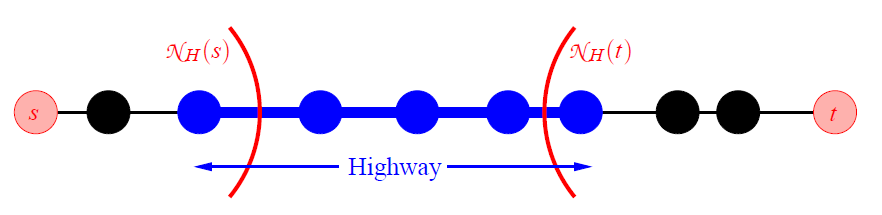
\includegraphics[scale=0.57]{highway.png}
            \caption{\label{fig:highway} Highway edges}
        \end{figure}

        Basically, the highway hierarchy is built by iterating the following procedure: \\

        \begin{center}
            $\text{input graph } G \xrightarrow{\text{select highway edges}} \text{highway network } G_1 \xrightarrow{\text{contract}} \text{contracted highway network } G'_1$
        \end{center}

        The selection of highway edges was already described. The contraction means two things:
        \begin{itemize}
            \item Take only the vertices with degree $\geq 2$
            \item Substitute paths whose internal vertices are of degree $2$ by one edge.
        \end{itemize}
        {\hfill}\\

        The removed parts of the graph are be called \textbf{components}. This way, we continually build smaller and smaller layers of the hierarchy (formed by highway networks - $G_1$), each time supplying $G'_1$ for the input of the next iteration. The lowest level is the original graph itself. \\

        On such a hierarchy (connected by vertical edges between vertices of the same type on neighboring levels of the hierarchy), a bidirectional Dijkstra's algorithm is run, with two constraints that can be informally described as: \\

        \begin{itemize}
            \item We do not follow one level of the hierarchy for too long
            \item Components of a given level of the hierarchy could be entered only when entering the level of the hierarchy itself
        \end{itemize}
        {\hfill}

        There are further optimizations described in the article, concerning speeding up the preprocessing, decreasing the size of the preprocessed information and the time of the query. \\

        \subsection{Route Planning in Road Networks}
        \label{subsec:routeplandiz}

        \textbff{Author(s): } Dominik Schultes \\
        \textbff{Year: }2008\\
        \textbff{Institution(s): }Universitat Karlsruhe

        \subsection{TRANSIT Ultrafast Shortest-Path Queries with Linear-Time Preprocessing}
        \label{subsec:transit}

        \textbff{Author(s): }
        \begin{itemizesp}
            \item Holger Bast
            \item Stefan Funke
            \item Domagoj Matijevic
        \end{itemizesp}
        \textbff{Year: }2006 \\
        \textbff{Institution(s): } Max-Planck-Institut fur Informatik, Saarbrucken, Germany\\
        {\hfill}\\
        \textbff{Concern:} The article presents a simple, yet very effective method for point-to-point shortest path queries in road networks, based on a precomputation of distances among a small set of so called ``transit nodes''. Upon query, the Dijkstra's algorithm is completely replaced by a few table look-ups, yielding impressive speed-ups in computation (6 orders of magnitude against the classical Dijkstra's algorithm).\\

        \textbff{Outline:} A simple, \textbf{basic idea} is quickly explained, then \textbf{related work} is compared to the proposed TRANSIT method. The \textbf{algorithm} is then described, mostly its preprocessing phase. \textbf{Modifications} that improve the efficiency are further considered and \textbf{experiments} are conducted before \textbf{concluding}. \\

        The surprisingly simple and effective idea is the following: \\

        A small set of \textbf{transit nodes} is first computed, that would cover all long-enough shortest paths in the graph (note a similarity with the approach in ~\cite{highwaydim10}). Then, for each vertex, a set of the closest transit nodes (so called \textbf{access nodes}) will be computed. The algorithm stores all the pair-wise distances among the transit nodes and for every node, the distances to its access nodes. This will not be too much, as for a road network of US (24 million nodes), the number of transit nodes turned out to be about 10000 and number of access nodes 10 on average (per vertex). \\

        A heuristics (e.g. air distance) is used to determine, if a posed query for distance between $x$ and $y$ is local, or not. In the latter case, all pairs of access nodes of $x$ and $y$ are considered and the one that minimizes the total distance is output. In the former case, some other exact method is used to determine the shortest path (e.g. Dijkstra's algorithm). Most queries (99\%) are non-local, and thus require just a few table look-ups. \\

        A simple way of obtaining not only the length of the path, but also the path itself is presented as well. \\

        \subsection{In Transit to Constant Time Shortest-Path Queries in Road Networks}
        \label{subsec:transithh}

        \textbff{Author(s): }
        \begin{itemizesp}
            \item Holger Bast
            \item Stefan Funke
            \item Domagoj Matijevic
            \item Peter Sanders
            \item Dominik Schultes
        \end{itemizesp}
        \textbff{Year: } 2007 \\
        \textbff{Institution(s): } \\
        \begin{itemizesp}
            \item Universitat Karlsruhe
            \item Max-Planck-Institut fur Informatik
        \end{itemizesp}

    \pagebreak
    \section{Time-dependent routing}

        \subsection{Time-Dependent SHARC-Routing}
        \label{subsec:sharc}

        \textbff{Author(s): } Daniel Delling \\
        \textbff{Year: }2008\\
        \textbff{Institution(s): }Universitat Karlsruhe

        \subsection{Time Dependent Contraction Hierarchies - Basic Algorithmic Ideas}
        \label{subsec:tchbasicalgideas}

        \textbff{Author(s): } Peter Sanders \\
        \textbff{Year: }2008\\
        \textbff{Institution(s): }Universitat Karlsruhe

        \subsection{Time-Dependent Contraction Hierarchies}
        \label{subsec:timedepch}

        \textbff{Author(s): }
        \begin{itemizesp}
            \item Gernot Veit Batz
            \item Daniel Delling
            \item Peter Sanders
            \item Christian Vetter
        \end{itemizesp}
        \textbff{Year: }2009\\
        \textbff{Institution(s): }Universitat Karlsruhe

    \pagebreak
    \section{Timetables related}

        \subsection{Experimental comparison of shortest path approaches for timetable}
        \label{subsec:compshpathapp}

        \textbff{Author(s): }
        \begin{itemizesp}
            \item Evangelia Pyrga
            \item Frank Schulz
            \item Dorothea Wagner
            \item Christos Zaroliagis
        \end{itemizesp}
        \textbff{Year: }2004 \\
        \textbff{Institution(s): }
        \begin{itemizesp}
            \item University of Karlsruhe
            \item University of Patras
        \end{itemizesp}

        \subsection{Engineering Time-Expanded Graphs for Faster Timetable Information}
        \label{subsec:engtimeexp}

        \textbff{Author(s): }
        \begin{itemizesp}
            \item Daniel Delling
            \item Thomas Pajor
            \item Dorothea Wagner
        \end{itemizesp}
        \textbff{Year: }2008 \\
        \textbff{Institution(s): } University of Karlsruhe \\
         {\hfill}\\
        \textbff{Concern:} This article studies quickest connection problem (earliest arrival problem) in time-expanded graphs. An extension of the model is presented, that takes transfers into account. It is then further preprocessed and optimized, so that once a (specifically adjusted) Dijsktra's algorithm is run on such a graph, it would correctly and effectively find the best connection. Existing speed-up techniques - Arc-Flags and ALT - which were designed for road networks are adapted for time-expanded graphs to yield a maximum speed-up factor of cca 56 against the classic Dijkstra's algorithm. \\

        \textbff{Outline:} Article gives a brief \textbf{preliminary} and a definition of the time-expanded model. Subsequently, this \textbf{model is further refined} by bypassing unnecessary nodes, remodeling stations and introducing parameters that control this fine-tuning - still in the phase of preprocessing. Two \textbf{speed-up techniques} using Dijkstra's algorithm are then considered. First one - Node-blocking - devised by authors, is tailored for time-expanded graphs and tries to prune from the search the unnecessary branches of the computation. The second one is an adaptation of a combination of Arc-Flags and ALT, two techniques designed for road networks. Quite extensive \textbf{experiments} form much of the last part. \\

        Several notes:
        \begin{itemize}
          \item It was left as an open point, how to handle updates in case of train (or carrier) delays, as updating time-expanded graphs is expensive
          \item Other techniques for road networks, like Highway Hierarchies, Contraction Hierarchies were considered, but their adaptation was said to be ``too challenging''
          \item A speed-up of 56 is not a bad achievement, but compared to speed-ups achieved in road networks (about $3$ million for Transit nodes combined with Edge-flags), one can wonder about possible improvements. However, speeding-up computation in time-dependent settings is much complicated, at least using techniques primarily devised for static routing.
        \end{itemize}

        \subsection{Using Multi-level Graphs for Timetable Information in Railway Systems }
        \label{subsec:multilevelgr}

        \textbff{Author(s): }
        \begin{itemizesp}
            \item Frank Schulz
            \item Dorothea Wagner
            \item Christos Zaroliagis
        \end{itemizesp}
        \textbff{Year: }2002 \\
        \textbff{Institution(s): }
        \begin{itemizesp}
            \item University of Konstanz
            \item University of Patras
        \end{itemizesp}

        \subsection{Timetable Information: Models and Algorithms}
        \label{subsec:timetablemodelsalgs}

        \textbff{Author(s): }
        \begin{itemizesp}
            \item Matthias Muller-Hannemann
            \item Frank Schulz
            \item Dorothea Wagner
            \item Christos Zaroliagis
        \end{itemizesp}
        \textbff{Year: }2006 \\
        \textbff{Institution(s): }
        \begin{itemizesp}
            \item Darmstadt University of Technology
            \item University of Karlsruhe
            \item University of Patras
        \end{itemizesp}
        {\hfill}\\
        \textbff{Concern:} The article considers various models and techniques how to deal with time-table information, primarily for the purpose of answering queries for shortest connection (solving earliest arrival problem - EAP). Time-expanded and time-dependent models are mostly discussed, both properly explained and later extended to model realistic requirements (like transfer time, cheapest connections, etc...). For multi-criteria optimization, approach that looks for Pareto sets is considered. Comparison between time-expanded and time-dependent models is made, with the latter doing better at EAP while the former being more convenient for multi-criteria optimization. \\

        \textbff{Outline:} A short mention of \textbf{historical timetable information systems} (TRAINS, ARIADNE) precedes the \textbf{definitions} (time-expanded/dependent models). Next, how Dijkstra's algorithm works with individual models is explained. The \textbf{models are then extended} to take into account realistic situations and requirements. The \textbf{multi-criteria queries} are considered and the \textbf{performance} of individual models is reviewed, summarizing the experimental results of several cited studies. The final part \textbf{concludes}. \\

        We will now introduce a few definitions, to make things clearer. \\

        \def\deftimetable{\textbf{A timetable on a given graph $G$} is a set $T_{G} = \{(x, y, p, q)|(x, y) \in E_{G}, \; p, q \in N, \; p < q \}$. An element of T is called an \textbf{elementary connection} and $x$ [$y$] and $p$ [$q$] are the \textbf{departure [arrival] node} and \textbf{time}. Graph $G$ is the \textbf{underlying graph} of timetable $T$.}\deftimetable \\

        \begin{table}[h!]{
            \small
            \begin{tabular}{c|c|c|c}
                %legend
                \hline
                    \rowcolor{tablehead}
                    \multicolumn{2}{>{\columncolor{tablehead}}c|}{\textbf{Place}} & \multicolumn{2}{>{\columncolor{tablehead}}c}{\textbf{Time}} \\
                    \hline
                    \rowcolor{tablehead}
                    \textbf{From} & \textbf{To} & \textbf{Departure} & \textbf{Arrival} \\
                %data
                \hline
                    A & B & 10:00 & 10:45 \\
                    A & B & 11:00 & 11:45 \\
                    A & B & 12:00 & 12:45 \\
                    A & C & 9:30 & 10:00 \\
                    A & C & 10:15 & 10:45 \\
                    C & D & 11:00 & 11:30 \\
                    C & D & 13:00 & 13:30 \\
                    C & D & 12:20 & 12:35 \\
                    C & D & 12:40 & 12:55 \\
                    C & D & 13:00 & 13:15 \\
                    C & B & 12:20 & 12:50 \\
                    C & B & 13:30 & 14:00 \\
                    D & A & 13:00 & 14:00 \\
            \end{tabular}}
            \caption{\label{tab:timetable01} An example of a timetable}
            \normalsize
        \end{table}

        \begin{figure}[h!]
            \begin{center}
                \inputTikZ{./tikzpics/basegraph}
            \end{center}
            \caption{\label{fig:underlying01} Underlying graph of the timetable in table ~\ref{tab:timetable01}}
        \end{figure}

        \def\defconnection{\textbf{A connection from $x$ to $y$ in a given timetable $T_{G}$} is a sequence of \emph{elementary connections} $e_{1}, e_{2}, ..., e_{k}, \; k \geq 1, \; e_{i} = (x_{i}, y_{i}, p_{i}, q_{i})$, such that $x_{0} = x$, $x_{k} = y$ and $\forall i \in \{2, ..., k\}: (x_{i} = y_{i - 1}, \; p_{i} \geq q_{i - 1})$. Connection \textbf{starts} at the \emph{departure time} $p_{1}$. \textbf{Size (length)} of the connection is $q_{k} - p_{1}$.}\defconnection \\

        The main problem dealt with is the so called \def\defeap{\textbf{earliest arrival problem (EAP)}: given a graph $G$, two of its vertices $x \neq y$, time $t$ and a timetable $T_{G}$ on the graph $G$, what is the shortest connection from $x$ to $y$ that starts at a time $s \geq t$. }\defeap Let us now look at the two models. \\

        \def\deftimeexpanded{Let $T$ be a timetable on $G$. \textbf{Time-expanded graph} from $T$ is an oriented graph $G_{T}$ whose vertices are pairs $[v, t], v \in G$ and $\exists (x, y, p, q) \in T$ such that $p = t$ or $q = t$. Edges of $G_{T}$ are formed by
        \begin{enumerate}
            \item $([x, p], [y, q]), ;\ \forall (x, y, p, q) \in T$ - connection edges
            \item $([x, p], [x, q]), [x, p], [x, q] \in V_{G_{T}}, p < q$ and $\not \exists [x, r] \in V_{G_{T}}: p < r < q$. - waiting edges (e.g. waiting for a train in a station)
        \end{enumerate}
        Weight $w$ of any edge $((x, p), (y, q))$ in $E_{G_{T}}$ is $w((x, p), (y, q)) = q - p$.}\deftimeexpanded \\

        \begin{figure}[h!]
            \scriptsize
            \begin{center}
                \inputTikZ{./tikzpics/timedependent}
            \end{center}
            \caption{\label{fig:timeexp01} Time-dependent graph of the timetable in table ~\ref{tab:timetable01}}
        \end{figure}

        \begin{figure}[h!]
            \scriptsize
            \begin{center}
                \inputTikZ{./tikzpics/timeexpanded}
            \end{center}
            \caption{\label{fig:timeexp01} Time-expanded graph from the timetable in table ~\ref{tab:timetable01}}
        \end{figure}

        \def\deftimedependent{Let $T$ be a timetable on $G$. \textbf{Time-dependent graph} of $T$ is an oriented graph $G_{T}$ whose vertices are $v \in G$. As for edges, $(u, v) \in E_{G_{T}} \iff \exists (u, v, p, q) \in T$. Weight $w$ of any edge in $E_{G_{T}}$ is defined during the run of the specific algorithm. }\deftimedependent Another point of view might be, that weights of the edges are functions, with time as their domain. \\

    \pagebreak
    \section{Others}

        \subsection{Complex networks: small-world, scale-free and beyond}
        \label{subsec:complexnetw}

        \textbff{Author(s): }
        \begin{itemizesp}
            \item Xiao Fan Wang
            \item Guanrong Chen
        \end{itemizesp}
        \textbff{Year: }2003 \\
        \textbff{Institution(s): }
        \begin{itemizesp}
            \item Department of Automation, Shanghai Jiao Tong University
            \item Central Queensland University, Australia
        \end{itemizesp}

    \pagebreak
    \section{Unclassified}

        \subsection{Reach for A*: Efficient Point-to-Point Shortest Path Algorithms}
        \label{subsec:reachforastar}

        \textbff{Author(s): }
        \begin{itemizesp}
            \item Andrew V. Goldberg
            \item Haim Kaplan
            \item Renato F. Werneck
        \end{itemizesp}
        \textbff{Year: }2006 \\
        \textbff{Institution(s): }
        \begin{itemizesp}
            \item Microsoft Research
            \item Tel Aviv University, Israel
            \item Department of Computer Science, Princeton University
        \end{itemizesp}

        \subsection{Car or Public Transport--Two Worlds}
        \label{subsec:twoworlds}
        \textbff{Author(s): } Hannah Bast
        \textbff{Year: }2009 \\
        \textbff{Institution(s): } Max-Planck-Institute for Informatics

    %---------------------------------------------------------------------
    %   main definitions
    %---------------------------------------------------------------------
    \section{List of main definitions}
        \begin{enumerate}
\ifmine
            \item \defspanner
            \item \defgirth
\fi
            \item \defdistlab
            \item \defbigrn
            \item \defseparator
            \item \defhd
            \item \deftimetable
            \item \defconnection
            \item \defeap
            \item \deftimeexpanded
            \item \deftimedependent
        \end{enumerate}

    %---------------------------------------------------------------------
    %   main results
    %---------------------------------------------------------------------
    \section{List of main results}
        \begin{enumerate}
            \item \resthzwck
\ifmine
            \item \resspangirth
            \item \resgirthtwok
            \item \reseveryspanner
            \item \reserdos
\fi
            \item \resseparator
            \item \restimelabelgeneral
        \end{enumerate}

    %---------------------------------------------------------------------
    %   main DO methods
    %---------------------------------------------------------------------
    \section{List of main DO methods}
        \begin{enumerate}
            \item Distance oracle of \textbf{Thorup and Zwick}.
            \begin{itemize}
                \item for general graphs
                \item \emph{preprocessing} - $\mathcal{O}(kmn^{1/k})$, \emph{size} - $\mathcal{O}(kn^{1 + 1/k})$, \emph{query time} - $\mathcal{O}(k)$, \emph{stretch} - $2k - 1$
            \end{itemize}
            \item Distance oracle of \textbf{Christian Sommer} for general graphs
            \begin{itemize}
                \item for general graphs
                \item based on random sampling and graph Voronoi duals
                \item longer query time decreases stretch
            \end{itemize}
            \item Distance labeling of \textbf{Gavoille}
            \begin{itemize}
                \item for graphs with $r(n)-separator$
                \item \emph{preprocessing} - depends, \emph{size} - $\mathcal{O}(n R(n) \log W + n \log^{2} n)$, \emph{query time} - $\mathcal{O}(\log n)$, \emph{stretch} - $1$
            \end{itemize}
            \item \textbf{Highway hierarchies}
            \begin{itemize}
                \item suitable for road networks
                \item based on hierarchies, shortcuts
                \item speed-up of 2000 against Dijkstra's algorithm
            \end{itemize}
            \item \textbf{Transit-node routing}
            \begin{itemize}
                \item suitable for road networks
                \item based on shortcuts, table-lookups
                \item speed-up of 1000000 against Dijkstra's algorithm
            \end{itemize}
            \item \textbf{Contraction hierarchies}
            \begin{itemize}
                \item suitable for road networks
                \item based on shortcuts, node contractions
                \item speed-up of 40000 against Dijkstra's algorithm
            \end{itemize}
            \item \textbf{Sketch-based distance oracle}
            \begin{itemize}
                \item suitable for web network, social networks
                \item based on landmarks
                \item \item \emph{preprocessing} - $O(k \cdot n^2)$, \emph{size} - $k n \log n$, \emph{query time} - $O(\log n)$, \emph{stretch} - for $k=\Theta (n^{1/c}polylog(n))$, stretch is $2c - 1$ \emph{whp}.
            \end{itemize}
        \end{enumerate}

    %---------------------------------------------------------------------
    %   bibliography
    %---------------------------------------------------------------------
    \pagebreak
    \bibliographystyle{is-alpha}
    %compile latex, bibtex, latex, latex
    \bibliography{../bibl}{}
\end{document}
